\section{可变参数类模板}
类模板也可以有数量可变的模板参数,这是构建标准库中某些类型类别(如tuple和variant)的关键。本节中,将了解如何为tuple类编写一个简单的实现。tuple是一种表示固定大小的异构值集合的类型。

实现可变函数模板时,使用了带有两个重载的递归模式,一个用于一般情况,另一个用于结束递归。除了为此目的需要使用特化外,可变参数类模板也必须采用相同的方法。下面是一个tuple类的最小实现:

\begin{cppcode}
template <typename T, typename... Ts>
struct tuple
{
	tuple(T const& t, Ts const &... ts)
	: value(t), rest(ts...)
	{
	}

	constexpr int size() const { return 1 + rest.size(); }
	
	T value;
	tuple<Ts...> rest;
};

template <typename T>
struct tuple<T>
{
	tuple(const T& t)
	: value(t)
	{
	}

	constexpr int size() const { return 1; }
	
	T value;
};
\end{cppcode}

第一个类是主模板,有两个模板参数:一个类型模板和一个参数包。所以,至少必须为实例化该模板指定一种类型。主模板元组有两个成员变量:value,类型为T, rest的类型为tuple<Ts...>,这是模板其余参数的扩展。说明包含N个元素的元组将包含第一个元素和另一个tuple;这第二个tuple,依次包含第二个元素和另一个tuple;这第三个嵌套tuple包含其余内容。这种模式一直持续下去,直到得到只有一个元素的tuple,这是由偏特化tuple<T>定义。与主模板不同,此特化不聚合另一个tuple对象。

可以使用这个简单的实现来编写如下代码:

\begin{cppcode}
tuple<int> one(42);
tuple<int, double> two(42, 42.0);
tuple<int, double, char> three(42, 42.0, 'a');

std::cout << one.value << '\n';
std::cout << two.value << ','
          << two.rest.value << '\n';
std::cout << three.value << ','
          << three.rest.value << ','
          << three.rest.rest.value << '\n';
\end{cppcode}

虽然可行,但需要通过rest成员访问元素,例如three.rest.rest.value,还是很繁琐的。而且tuple的元素越多,用这种方式写代码就越难。因此,我们希望使用一些辅助函数来简化tuple元素的访问:

\begin{cppcode}
std::cout << get<0>(one) << '\n';
std::cout << get<0>(two) << ','
          << get<1>(two) << '\n';
std::cout << get<0>(three) << ','
          << get<1>(three) << ','
          << get<2>(three) << '\n';
\end{cppcode}

get<N>是一个可变参函数模板,接受一个tuple作为参数,并返回对元组中第N个索引处元素的引用。其原型可能如下所示:

\begin{cppcode}
template <size_t N, typename... Ts>
typename nth_type<N, Ts...>::value_type & get(tuple<Ts...>& t);
\end{cppcode}

模板参数是元组类型的索引和形参包,但其实现需要一些帮助器类型。首先,需要了解tuple中第N个下标处元素的类型。可以在以下nth_type可变类型模板的帮助下进行检索:

\begin{cppcode}
template <size_t N, typename T, typename... Ts>
struct nth_type : nth_type<N - 1, Ts...>
{
	static_assert(N < sizeof...(Ts) + 1,
	              "index out of bounds");
};

template <typename T, typename... Ts>
struct nth_type<0, T, Ts...>
{
	using value_type = T;
};
\end{cppcode}

同样,有一个主模板,使用递归继承和索引0的特化。特化为第一个类型模板定义了一个名为value_type的别名(是模板参数列表的头),此类型仅用作确定tuple元素类型的机制,需要另一个可变参数类模板来检索值:

\begin{cppcode}
template <size_t N>
struct getter
{
	template <typename... Ts>
	static typename nth_type<N, Ts...>::value_type&
	get(tuple<Ts...>& t)
	{
		return getter<N - 1>::get(t.rest);
	}
};

template <>
struct getter<0>
{
	template <typename T, typename... Ts>
	static T& get(tuple<T, Ts...>& t)
	{
		return t.value;
	}
};
\end{cppcode}

可以看到相同的递归模式,有一个主模板和一个显式特化。类模板称为getter,只有一个模板参数,这是非类型模板参数,这个参数表示要访问的tuple元素的索引。这个类模板有一个名为get的静态成员函数,是一个可变参数函数模板。主模板中的实现以tuple的其余成员作为参数调用get函数,并且显式特化的实现会返回对元组成员值的引用。

定义了这些之后,现在可以为辅助可变参数函数模板get提供一个实现。这个实现依赖于getter类模板,并调用其get可变参数函数模板:

\begin{cppcode}
template <size_t N, typename... Ts>
typename nth_type<N, Ts...>::value_type &
get(tuple<Ts...>& t)
{
	return getter<N>::get(t);
}
\end{cppcode}

若这个例子有点复杂,那么对其一步步地分析可能会有助于读者们更好地理解其工作原理。先从以下片段开始:

\begin{cppcode}
tuple<int, double, char> three(42, 42.0, 'a');
get<2>(three);
\end{cppcode}

使用cppinsights.io Web工具来检查,这个代码段中发生的模板实例化。首先要查看的是类模板元组,有一个主模板和几个特化:

\begin{cppcode}
template <typename T, typename... Ts>
struct tuple
{
	tuple(T const& t, Ts const &... ts)
	   : value(t), rest(ts...)
	{ }
	
	constexpr int size() const { return 1 + rest.size(); }
	
	T value;
	tuple<Ts...> rest;
};

template<> struct tuple<int, double, char>
{
	inline tuple(const int & t,
	             const double & __ts1, const char & __ts2)
	: value{t}, rest{tuple<double, char>(__ts1, __ts2)}
	{}
	
	inline constexpr int size() const;
	
	int value;
	tuple<double, char> rest;
};

template<> struct tuple<double, char>
{
	inline tuple(const double & t, const char & __ts1)
	: value{t}, rest{tuple<char>(__ts1)}
	{}
	
	inline constexpr int size() const;
	
	double value;
	tuple<char> rest;
};

template<> struct tuple<char>
{
	inline tuple(const char & t)
	: value{t}
	{}
	
	inline constexpr int size() const;
	
	char value;
};

template<typename T>
struct tuple<T>
{
	inline tuple(const T & t) : value{t}
	{ }
	
	inline constexpr int size() const
	{ return 1; }
	
	T value;
};
\end{cppcode}

tuple<int, double, char>结构包含一个int和一个tuple<double, char>;tuple<double, char>包含一个double和一个tuple<char>;tuple<char>又包含一个char值,最后一个类表示元组的递归定义的结束。可以用以下图形表示:

\begin{center}
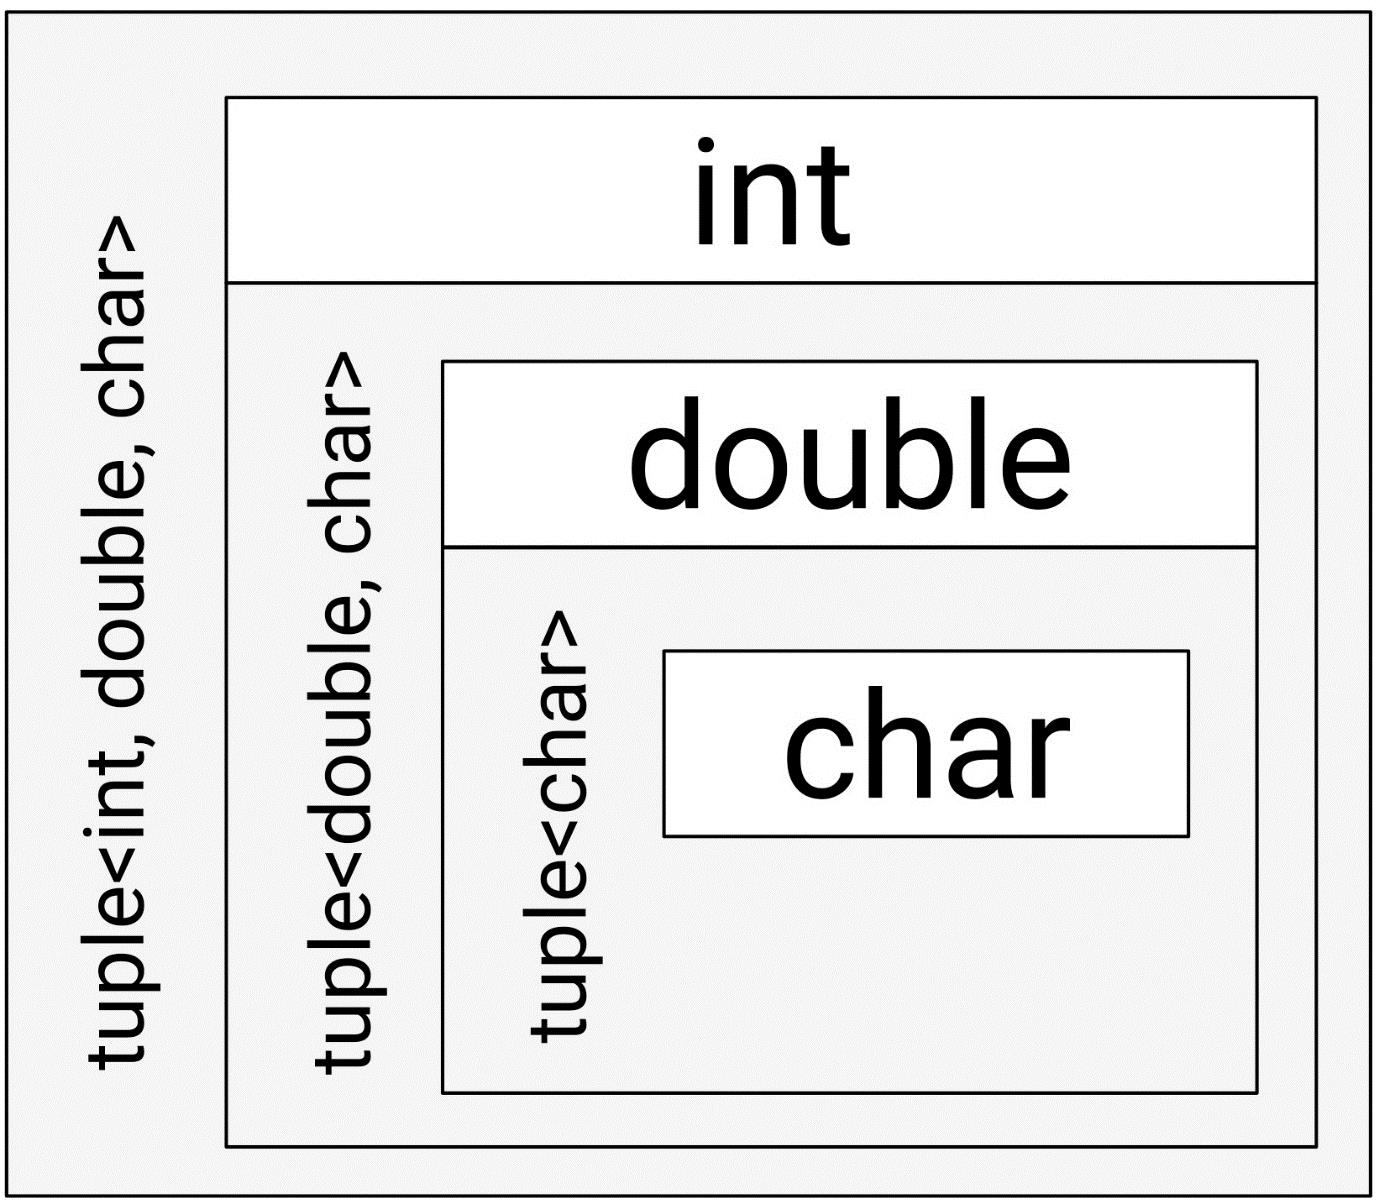
\includegraphics[width=0.4\textwidth]{images/1.png}\\
图3.1 - 元组的示例
\end{center}

接下来,是nth_type类模板,一个主模板和几个特化:

\begin{cppcode}
template <size_t N, typename T, typename... Ts>
struct nth_type : nth_type<N - 1, Ts...>
{
	static_assert(N < sizeof...(Ts) + 1,
	              "index out of bounds");
};

template<>
struct nth_type<2, int, double, char> :
   public nth_type<1, double, char>
{ };

template<>
struct nth_type<1, double, char> : public nth_type<0, char>
{ };

template<>
struct nth_type<0, char>
{
	using value_type = char;
};

template<typename T, typename ... Ts>
struct nth_type<0, T, Ts...>
{
	using value_type = T;
};
\end{cppcode}

nth_type<2, int, double, char>特化派生自nth_type<1, double, char>,而nth_type<1, double, char>又派生自nth_type<0, char>,nth_type<0, char>是层次结构中的最后一个基类(递归层次结构的末尾)。

nth_type结构体用作getter辅助类模板中的返回类型,实例化如下所示:

\begin{cppcode}
template <size_t N>
struct getter
{
	template <typename... Ts>
	static typename nth_type<N, Ts...>::value_type&
	get(tuple<Ts...>& t)
	{
		return getter<N - 1>::get(t.rest);
	}
};

template<>
struct getter<2>
{
	template<>
	static inline typename
	nth_type<2UL, int, double, char>::value_type &
	get<int, double, char>(tuple<int, double, char> & t)
	{
		return getter<1>::get(t.rest);
	}
};

template<>
struct getter<1>
{
	template<>
	static inline typename nth_type<1UL, double,
	                                char>::value_type &
	get<double, char>(tuple<double, char> & t)
	{
		return getter<0>::get(t.rest);
	}
};
template<>
struct getter<0>
{
	template<typename T, typename ... Ts>
	static inline T & get(tuple<T, Ts...> & t)
	{
		return t.value;
	}

	template<>
	static inline char & get<char>(tuple<char> & t)
	{
		return t.value;
	}
};
\end{cppcode}

最后,检索tuple元素值的get函数模板定义:

\begin{cppcode}
template <size_t N, typename... Ts>
typename nth_type<N, Ts...>::value_type &
get(tuple<Ts...>& t)
{
	return getter<N>::get(t);
}

template<>
typename nth_type<2UL, int, double, char>::value_type &
get<2, int, double, char>(tuple<int, double, char> & t)
{
	return getter<2>::get(t);
}
\end{cppcode}

若有更多对get函数的调用,get的特化就会更多。例如,对于get<1>(3),将添加以下特化:

\begin{cppcode}
template<>
typename nth_type<1UL, int, double, char>::value_type &
get<1, int, double, char>(tuple<int, double, char> & t)
{
	return getter<1>::get(t);
}
\end{cppcode}

这个例子演示了如何使用用于一般情况的主模板,和一个用于可变参数递归的结束情况的特化来实现可变参数类模板。

这里使用关键字typename作为nth_type<N, Ts...>::value_type类型的前缀,是一个依赖类型。C++20中,这个不再必要,这个主题将在第4章中详细讨论。

由于实现可变参数模板通常是冗长且繁琐的,C++17标准添加了折叠表达式来进行简化。我们将在下一节中来探讨折叠表达式。


